\section{Parallelkinematische Maschinen Neugebauer}

\begin{itemize}
    \item kinematische Struktur
    \item Systematisierung anhand der Ordnungskriterien „Freiheitsgrad“, „Anzahl der Führungsketten“ und „Anzahl der Antriebe“ verwendet
\end{itemize}

\subsection{Struktursystematik}
Parallelkinematische Mechanismen sind – aus getriebetechnischer Sicht betrachtet – ungleichmäßig übersetzende Mechanismen. Hinsichtlich ihrer Funktion kann man zwischen Übertragungsgetrieben und Führungsgetrieben unterscheiden. Erstere dienen der Übertragung mechanischer Leistung, bei Letzteren wird ein Getriebeglied so geführt, dass es bestimmte Lagen einnimmt, bzw. dass seine Punkte bestimmte Bahnen, sog. Führungsbahnen, beschreiben [145, 146]. Eine aus energetischer Sicht untergeordnete Rolle spielt bei Führungsgetrieben deren Übertragungsfunktion. Mechanismen mit parallelen Strukturen werden den Führungsgetrieben zugeordnet. Da Getriebe nach ihren charakteristischen Bestandteilen eingeteilt werden können, gehören die hier interessierenden Mechanismen zu den Koppelgetrieben. Die eben betrachteten Kriterien geben den parallelkinematischen Mechanismen einen eindeutigen Platz innerhalb der Ordnung aller Getriebe. Parallelkinematiken sind Führungsgetriebe, bei denen die Arbeitsplattform über mindestens zwei angetriebene Führungsketten mit dem Gestell verbunden ist. \footcite[Vgl.][14]{Neugebauer2006}

\subsection{Grundstrukturen}

\begin{figure}[H]
    \centering
    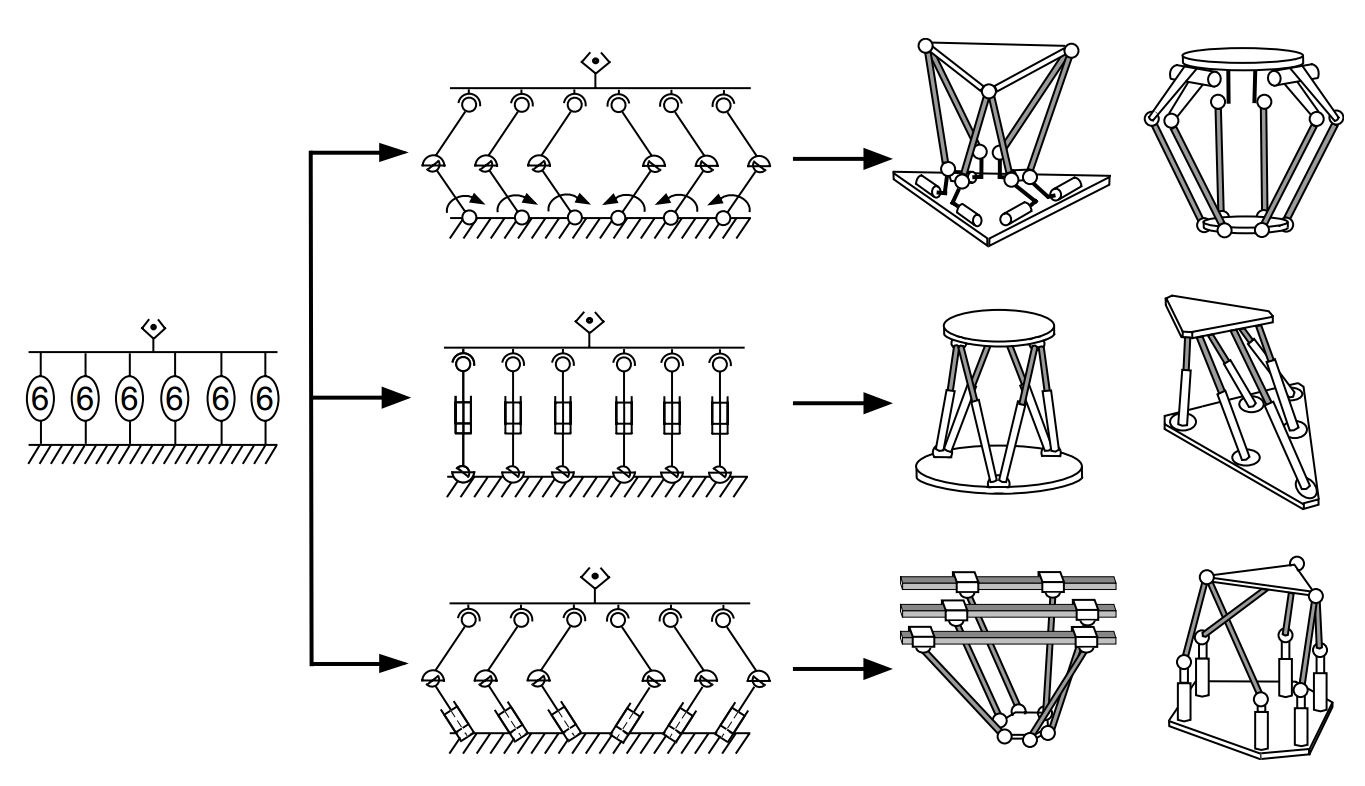
\includegraphics[width=\textwidth]{basics/aufbau/strukturentwicklung}
    \caption[Entwicklung einer Parallelkinematik]{Entwicklung einer Parallelkinematik: vom kinematischen Schema über das kinematische Prinzip zur kinematischen Struktur; Quelle: Neugebauer (2006), Parallelkinematische Maschinen}
    \label{fig:stab1}
\end{figure}

\begin{itemize}
    \item Alle Führungsketten haben genau einen Antrieb mit dem Freiheitsgrad Eins.
    \item Mindestens eine Führungskette hat mehr als einen Antrieb mit dem Freiheitsgrad Eins.
    \item Mindestens eine Führungskette hat keinen Antrieb.
\end{itemize}

Ausgehend von den Gleichungen (2.1) und (2.2) zur Bestimmung des Freiheitsgrades von Mechanismen werden die Mechanismen so abstrahiert, dass nur noch die Anzahl der Führungsketten FK und deren Freiheitsgrad F in die Berechnung eingehen. Der Freiheitsgrad F der Führungsketten wird berechnet aus dem Freiheitsgrad der Führungsketten gemäß Gln. (2.1) und (2.2) plus dem Gelenkfreiheitsgrad des Verbindungsgelenks zwischen Führungskette und Arbeitsplattform. Bei räumlichen Getrieben mit ebenen Teilgetrieben werden letztere gesondert behandelt. Sie werden als Ersatzgelenk mit dem entsprechenden Gelenkfreiheitsgrad in der Freiheitsgradberechnung des räumlichen Getriebes berücksichtigt.

\begin{figure}[H]
    \centering
    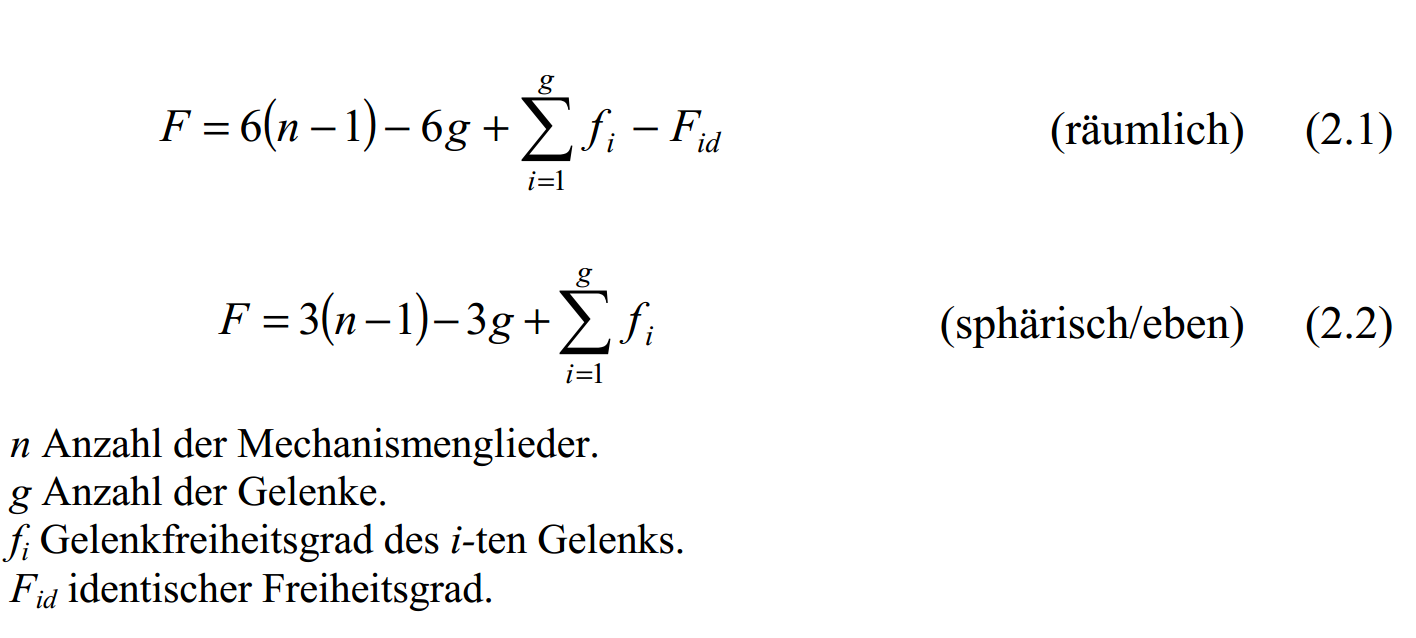
\includegraphics[width=\textwidth]{basics/aufbau/fk_gleichungen}
\end{figure}

Hinzuzufügen ist, dass Führungsketten mit F = 6 mindestens einen Antrieb haben müssen, da sie sonst für den Mechanismus ohne kinematische Bedeutung sind. \footcite[Vgl.][17]{Neugebauer2006}

\begin{figure}[H]
    \centering
    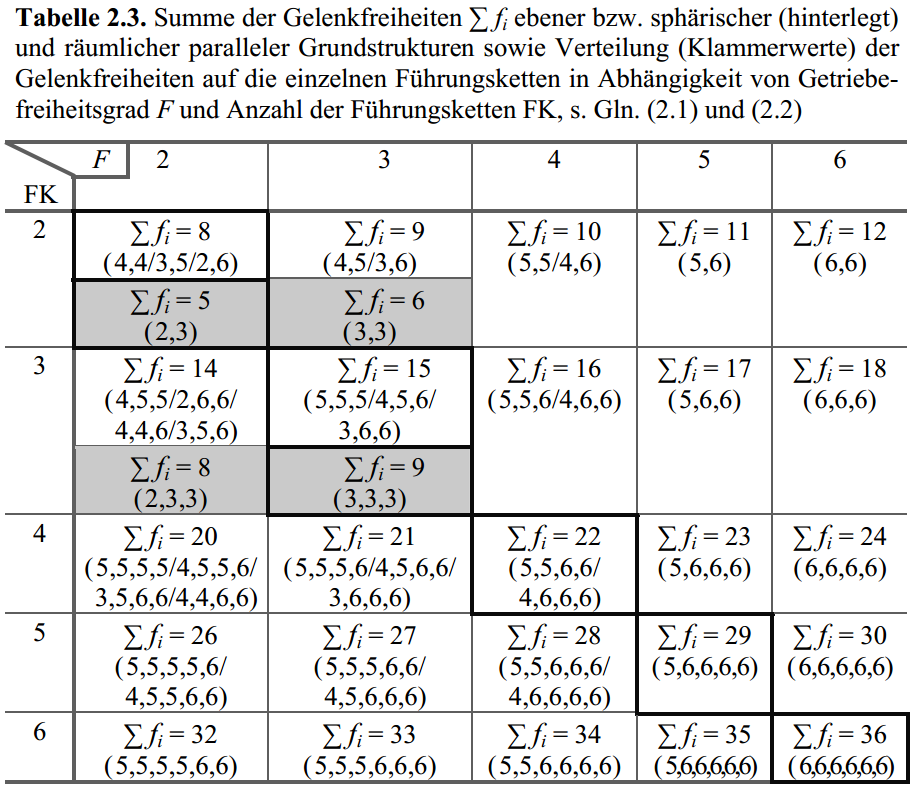
\includegraphics[width=\textwidth]{basics/aufbau/tab_gelenkfreiheiten}
\end{figure}

Parallele Strukturen, in denen jede Führungskette genau einen Antrieb mit dem Freiheitsgrad Eins enthält, werden „vollparallel“ genannt und entsprechen in Tabelle 2.3. allen Schemata entlang der Diagonalen. 

Für die Grundformen der häufig in Parallelkinematiken zur Anwendung kommenden Gelenke werden im Weiteren Bezeichnungen verwendet, die im Wesentlichen auf die z. B. in [30] und [145, 146] vorgestellten zurückgehen:

\begin{itemize}
    \item Drehgelenk (D)
    \item Drehschubgelenk (DS)
    \item Kardangelenk (DD)
    \item Kugelgelenk ($D_3$)
    \item Schubgelenk (S)
\end{itemize}

\begin{figure}[H]
    \centering
    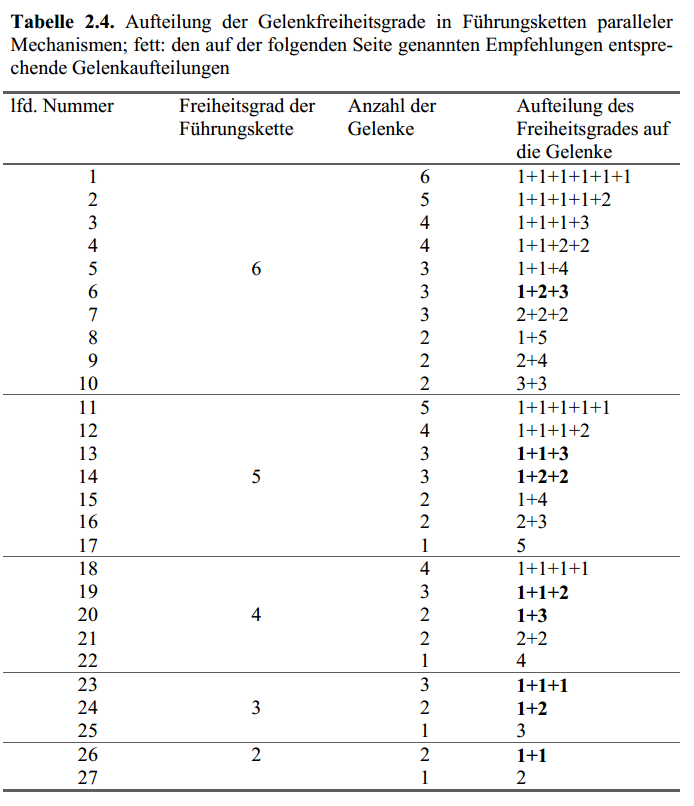
\includegraphics[width=\textwidth]{basics/aufbau/fk_empfehlungen}
\end{figure}

Für die Gestaltung der Führungsketten, d. h. die konkrete Verteilung der Gelenkfreiheiten, sind beliebige Varianten denkbar. Entsprechend Tabelle 2.4. kommen Führungsketten, deren Freiheitsgrad die Bedingung 2 kleiner gleich F kleiner gleich 6 erfüllt, in Betracht. Nachfolgend sind alle Möglichkeiten der Verteilung der Gelenkfreiheiten innerhalb der Führungsketten aufgeführt. Die Reihenfolge kann variiert werden. Der nächste Entwicklungsschritt ist die Zuordnung konkreter Gelenke zu den Gelenkfreiheiten. Dabei ist zu beachten, dass in der bisher vorgestellten Systematik auch solche Grundstrukturen erfasst sind, die einerseits aufgrund einer ungünstigen Gelenkanordnung nicht lauffähig oder andererseits einer zu großen Anzahl von Gelenken wegen praktisch irrelevant sind. Um aber dennoch dem Konstrukteur mit der Entwicklungssystematik ein handhabbares und hilfreiches Werkzeug verfügbar zu machen, müssen diese Grundstrukturen von den praktisch zweckmäßigen und nutzbaren unterschieden werden. Insoweit können folgende einschränkende Forderungen an die konstruktive Ausführung von Führungsketten als Empfehlung geltend gemacht werden:

\begin{itemize}
    \item Aufgrund der Forderung nach linearer Unabhängigkeit der Gelenkachsen dürfen im ebenen Fall maximal zwei und im räumlichen Fall maximal drei Schubgelenke in einer Gelenkkette vorhanden sein.
    \item Die Antriebe müssen gestellnah angeordnet werden, um die zu bewegende Maschinenmasse weitestgehend zu reduzieren. Als Antriebsgelenke sollen Gelenke mit dem Freiheitsgrad Eins verwendet werden.
    \item Die einzelnen Gelenkketten sollten gleichartig aufgebaut sein, um den konstruktiven Aufwand und die Fertigungskosten zu minimieren.
    \item Bei passiven Gelenken sind Drehgelenke gegenüber Schubgelenken aufgrund des geringeren konstruktiven Aufwands zu bevorzugen. Außerdem ist bei passiven Schubgelenken die Klemmgefahr zu beachten. Es sollten nur Gelenke mit einem Gelenkfreiheitsgrad kleiner Vier zum Einsatz kommen.
    \item Eine Führungskette sollte einschließlich der Anschlussgelenke an Plattform und Gestell nur drei Gelenke enthalten, da sonst die Steifigkeit zu gering ist und Fehler durch seriellen Aufbau der Maßketten (Summenfehler) auftreten.
\end{itemize}

Bei mehrfach angetriebenen Führungsketten sind Lösungsmöglichkeiten auf Basis ebener Teilstrukturen zu bevorzugen (Möglichkeit, alle Antriebe gestellnah anzuordnen, bzw. kein serieller Aufbau). Die Antriebe sind so anzuordnen, dass jede Führungskette mindestens eine Freiheit der Plattform bindet. Bezogen auf Führungsketten mit F = 6 bedeutet dies, dass sie mindestens einen Antrieb enthalten müssen. Prinzipiell ist zwischen zwangführenden und nicht-zwangführenden Führungsketten zu unterscheiden. Letztere schränken die Bewegung des Endeffektors nicht ein. Im ebenen Fall sind dafür drei und im räumlichen Fall sechs Gelenkfreiheiten notwendig.

\begin{itemize}
    \item Gelenke $f_i = 2$ Drehschubgelenk; Kardangelenk
    \item Gelenke $f_i = 3$ Kugelgelenk
\end{itemize}